%%%%%%%%%%%%%%%%%%%%%%%%%%%%%%%%%%%%%%%
% Programming/Coding Assignment
% LaTeX Template
%
% This template has been downloaded from:
% http://www.latextemplates.com
%
% Original author:
% Ted Pavlic (http://www.tedpavlic.com)
%
% Note:
% The \lipsum[#] commands throughout this template generate dummy text
% to fill the template out. These commands should all be removed when 
% writing assignment content.
%
% This template uses a Perl script as an example snippet of code, most other
% languages are also usable. Configure them in the "CODE INCLUSION 
% CONFIGURATION" section.
%
%%%%%%%%%%%%%%%%%%%%%%%%%%%%%%%%%%%%%%%%%

%----------------------------------------------------------------------------------------
%	PACKAGES AND OTHER DOCUMENT CONFIGURATIONS
%----------------------------------------------------------------------------------------

\documentclass[a4paper]{article}

\usepackage{fancyhdr} % Required for custom headers
\usepackage{lastpage} % Required to determine the last page for the footer
\usepackage{extramarks} % Required for headers and footers
\usepackage[usenames,dvipsnames]{color} % Required for custom colors
\usepackage{graphicx} % Required to insert images
\usepackage{listings} % Required for insertion of code
\renewcommand*{\lstlistingname}{代码} % change "Listing <ref> to 代码 <ref>
\usepackage{courier} % Required for the courier font
\usepackage{lipsum} % Used for inserting dummy 'Lorem ipsum' text into the template

\usepackage[UTF8]{ctex} % Required for Chinese character
\usepackage{tocloft} % Required for beautiful toc
\usepackage[colorlinks]{hyperref} % Required for clickable toc
\hypersetup{
    colorlinks=false,
    citecolor=red,
    filecolor=black,
    linkcolor=blue,
    urlcolor=black,
    linkbordercolor	= {1 0 0}
}
\usepackage[title]{appendix} % Required for appendix
\usepackage{float}
\usepackage{amsmath} % used for \text{} in math formula


% used for beautiful table
\usepackage{booktabs} 
\usepackage[T1]{fontenc}
\usepackage{tabu}
\usepackage{longtable}
\usepackage[table]{xcolor}

\usepackage{algpseudocode}
\usepackage{algorithm}

\def\equationautorefname{式}%
\def\footnoteautorefname{脚注}%
\def\itemautorefname{项}%
\def\figureautorefname{图}%
\def\tableautorefname{表}%
\def\partautorefname{篇}%
\def\appendixautorefname{附录}%
\def\chapterautorefname{章}%
\def\sectionautorefname{节}%
\def\subsectionautorefname{小小节}%
\def\subsubsectionautorefname{subsubsection}%
\def\paragraphautorefname{段落}%
\def\subparagraphautorefname{子段落}%
\def\FancyVerbLineautorefname{行}%
\def\theoremautorefname{定理}%
\def\algorithmautorefname{算法}
% TODO:
\newcommand{\aref}[1]{\hyperref[#1]{附录~\ref{#1}}}

% Margins
\topmargin=-0.45in
\evensidemargin=0in
\oddsidemargin=0in
\textwidth=6.5in
\textheight=9.0in
\headsep=0.25in

\linespread{1.1} % Line spacing

% Set up the header and footer
\pagestyle{fancy}
\lhead{\hmwkAuthorName} % Top left header
\chead{\hmwkClass\ (\hmwkClassInstructor\ \hmwkClassTime): \hmwkTitle} % Top center head
\rhead{\firstxmark} % Top right header
\lfoot{\lastxmark} % Bottom left footer
\cfoot{} % Bottom center footer
\rfoot{Page\ \thepage\ of\ \protect\pageref*{LastPage}} % Bottom right footer
\renewcommand\headrulewidth{0.4pt} % Size of the header rule
\renewcommand\footrulewidth{0.4pt} % Size of the footer rule

\setlength\parindent{0pt} % Removes all indentation from paragraphs

%----------------------------------------------------------------------------------------
%	CODE INCLUSION CONFIGURATION
%----------------------------------------------------------------------------------------

\definecolor{MyDarkGreen}{rgb}{0.0,0.4,0.0} % This is the color used for comments
% \lstloadlanguages{c} % Load Perl syntax for listings, for a list of other languages supported see: ftp://ftp.tex.ac.uk/tex-archive/macros/latex/contrib/listings/listings.pdf
% \lstset{language=sql, % Use Perl in this example
%         frame=single, % Single frame around code
%         basicstyle=\small\ttfamily, % Use small true type font
%         keywordstyle=[1]\color{Blue}, % Perl functions bold and blue
%         keywordstyle=[2]\color{Purple}, % Perl function arguments purple
%         keywordstyle=[3]\color{Blue}\underbar, % Custom functions underlined and blue
%         identifierstyle=, % Nothing special about identifiers                                         
%         commentstyle=\usefont{T1}{pcr}{m}{sl}\color{MyDarkGreen}\small, % Comments small dark green courier font
%         stringstyle=\color{Purple}, % Strings are purple
%         showstringspaces=false, % Don't put marks in string spaces
%         tabsize=4, % 5 spaces per tab
%         %
%         % Put standard Perl functions not included in the default language here
%         % morekeywords={rand},
%         morekeywords={rand, go},
%         %
%         % Put Perl function parameters here
%         morekeywords=[2]{REAL},
%         %
%         % Put user defined functions here
%         morekeywords=[3]{},
%        	%
%         morecomment=[l][\color{Blue}]{...}, % Line continuation (...) like blue comment
%         numbers=left, % Line numbers on left
%         firstnumber=1, % Line numbers start with line 1
%         numberstyle=\tiny\color{Blue}, % Line numbers are blue and small
%         stepnumber=2, % Line numbers go in steps of 5,
%         firstnumber=1
% }

\lstloadlanguages{C++}
\lstdefinestyle{mycpp}{
    language=C++, % Use Perl in this example
    frame=single, % Single frame around code
    basicstyle=\small\ttfamily, % Use small true type font
    keywordstyle=[1]\color{Blue}, % Perl functions bold and blue
    keywordstyle=[2]\color{Purple}, % Perl function arguments purple
    keywordstyle=[3]\color{Blue}\underbar, % Custom functions underlined and blue
    keywordstyle=[4]\color{Aquamarine}, % Custom functions underlined and blue
    identifierstyle=, % Nothing special about identifiers                                         
    commentstyle=\usefont{T1}{pcr}{m}{sl}\color{MyDarkGreen}\small, % Comments small dark green courier font
    stringstyle=\color{Purple}, % Strings are purple
    showstringspaces=false, % Don't put marks in string spaces
    tabsize=4, % 5 spaces per tab
    %
    % Put standard Perl functions not included in the default language here
    % morekeywords={rand},
    morekeywords={go, REFERENCES, DATABASE, SCHEMA},
    %
    % Put Perl function parameters here
    morekeywords=[4]{np},
    %
    % Put user defined functions here
    morekeywords=[1]{self},
    morekeywords=[3]{},
    %
    morecomment=[l][\color{Blue}]{...}, % Line continuation (...) like blue comment
    numbers=left, % Line numbers on left
    firstnumber=1, % Line numbers start with line 1
    numberstyle=\tiny\color{Blue}, % Line numbers are blue and small
    stepnumber=2, % Line numbers go in steps of 5,
    firstnumber=1
}
% Creates a new command to include a perl script, the first parameter is the filename of the script (without .pl), the second parameter is the caption

\newcommand{\shfilescript}[3]{
\begin{itemize}
\item[]\lstinputlisting[caption=#2, label=lst:#1, language=sh]{#3}
\end{itemize}
}
\newcommand{\shscript}[3]{
\begin{itemize}
\item[]\begin{lstlisting}[label=lst:#1, caption=#2] #3 \end{lstlisting}
\end{itemize}
}

%----------------------------------------------------------------------------------------
%	DOCUMENT STRUCTURE COMMANDS
%	Skip this unless you know what you're doing
%----------------------------------------------------------------------------------------

% Header and footer for when a page split occurs within a problem environment
\newcommand{\enterProblemHeader}[1]{
\nobreak\extramarks{#1}{#1 见下页\ldots}\nobreak{} 
\nobreak\extramarks{接上页}{#1 见下页\ldots}\nobreak{}
}

% Header and footer for when a page split occurs between problem environments
\newcommand{\exitProblemHeader}[1]{
\nobreak\extramarks{接上页}{#1 见下页\ldots}\nobreak{}
\nobreak\extramarks{#1}{}\nobreak{}
}
% TODO:code here enable the number before section, but it disable the numbering of problems
%\setcounter{secnumdepth}{0} % Removes default section numbers
\newcounter{homeworkProblemCounter} % Creates a counter to keep track of the number of problems

\newcommand{\homeworkProblemName}{}
\newenvironment{homeworkProblem}[1][Problem \arabic{homeworkProblemCounter}]{ % Makes a new environment called homeworkProblem which takes 1 argument (custom name) but the default is "Problem #"
\stepcounter{homeworkProblemCounter} % Increase counter for number of problems
\renewcommand{\homeworkProblemName}{#1} % Assign \homeworkProblemName the name of the problem
\section{\homeworkProblemName} % Make a section in the document with the custom problem count
\enterProblemHeader{\homeworkProblemName} % Header and footer within the environment
}{
\exitProblemHeader{\homeworkProblemName} % Header and footer after the environment
}

\newcommand{\problemAnswer}[1]{ % Defines the problem answer command with the content as the only argument
\noindent\framebox[\columnwidth][c]{\begin{minipage}{0.98\columnwidth}#1\end{minipage}} % Makes the box around the problem answer and puts the content inside
}

\newcommand{\homeworkSectionName}{}
\newenvironment{homeworkSection}[1]{ % New environment for sections within homework problems, takes 1 argument - the name of the section
\renewcommand{\homeworkSectionName}{#1} % Assign \homeworkSectionName to the name of the section from the environment argument
\subsection{\homeworkSectionName} % Make a subsection with the custom name of the subsection
\enterProblemHeader{\homeworkProblemName\ [\homeworkSectionName]} % Header and footer within the environment
}{
\enterProblemHeader{\homeworkProblemName} % Header and footer after the environment
}


\newcommand{\codev}[1]{\textsf{#1}}
%----------------------------------------------------------------------------------------
%	NAME AND CLASS SECTION
%----------------------------------------------------------------------------------------

% table color
\definecolor{tableHeader}{RGB}{245, 245, 245}
\definecolor{tableLineOne}{RGB}{245, 245, 245}
\definecolor{tableLineTwo}{RGB}{224, 224, 224}
\newcommand{\tableHeaderStyle}{
    \rowfont{\leavevmode\color{white}\bfseries}
    \rowcolor{tableHeader}
}

%----------------------------------------------------------------------------------------

\newcommand{\hmwkTitle}{高性能计算\ \#实验4} % Assignment title
\newcommand{\hmwkDueDate}{Tuesday,\ November\ 20,\ 2018} % Due date
\newcommand{\hmwkClass}{16级计科\ 7班} % Course/class
\newcommand{\hmwkClassTime}{周二1-2节} % Class/lecture time
\newcommand{\hmwkClassInstructor}{张永东} % Teacher/lecturer
\newcommand{\hmwkAuthorName}{颜彬} % Your name
\newcommand{\hmwkAuthorId}{16337269} % Your id 

%----------------------------------------------------------------------------------------
%	TITLE PAGE
%----------------------------------------------------------------------------------------

\usepackage{titling}

\title{
\vspace{2in}
\textmd{\textbf{\hmwkClass:\ \hmwkTitle}}\\
\normalsize\vspace{0.1in}\small{Due\ on\ \hmwkDueDate}\\
\vspace{0.1in}\large{\textit{\hmwkClassInstructor\ \hmwkClassTime}}
\vspace{3in}
}

\author{\textbf{\LARGE{\hmwkAuthorName}} \\ \\ \textbf{\LARGE{\hmwkAuthorId}}}
\date{} % Insert date here if you want it to appear below your name
%----------------------------------------------------------------------------------------

\begin{document}
% \begin{titlingpage} % This is for ignore page number in first page. package titling

\maketitle

%----------------------------------------------------------------------------------------
%	TABLE OF CONTENTS
%----------------------------------------------------------------------------------------

% \setcounter{tocdepth}{2} % Uncomment this line if you don't want subsections listed in the ToC
% set depth in toc

% \renewcommand{\cftsecleader}{\cftdotfill{\cftdotsep}} % used for dots between <section> and <page>

\renewcommand{\contentsname}{Content} % force the word to be "content
\newpage
\tableofcontents
\addtocontents{toc}{~\hfill\textbf{Page}\par}
\newpage

% below are document body


% To have just one problem per page, simply put a \clearpage after each problem
\section{算法简介}
并行正则采样排序是一个并行排序算法。在算法运行的任意一个时刻,每个进程都不需要拥有全部
的数据。它可以解决对数据量极大的场景下的排序。\\

算法的最终结果是
\begin{itemize}
    \item 进程内,所有的数据有序
    \item 进程间,对任意进程$p_i,\ p_j\quad \text{s.t.}\ i < j$,都有i进程内的任意一个数
    小于j进程内的任意一个数。
\end{itemize}
于是数据被排列成全局有序。\\

在管理这些有序的数据时,可以选择一个进程作为主进程,
存储所有其他进程的第一个有序数。以该有序数作为分界线。
\section{算法步骤}
这里假设初始的全部数据都位于0号进程。实际上,算法也允许初始的数据分成p份位于p个进程中。
算法不需要p个进程中每个进程拥有的数据数量相等。\\

假设p代表进程数量,n代表待排序的数字总数。所有的$/$符号代表下取整的除法。
\subsection{均匀划分}\label{subsec:st1}
0号进程将所有的数据尽可能相等地分成p份,并分发到p个进程中。
设$$m = n \bmod p$$
则前n-m个进程获得$n/p$个数据,后m个进程获得$n/p + 1$个数据。
\subsection{局部排序}\label{subsec:localsort}
由于此时每个进程获得的局部数据是乱序的,故采用快速排序的方法来进行局部排序。可以证明,
在数据属于随机分布时,在大部分情况下快速排序都能获得较好的期望复杂度。
\subsection{正则采样}
每个进程从局部有序的数组中等间距地选取t个pivot。设$d_i$代表i号进程拥有的
数据的数量,$A_i$代表局部有序的数组。则进程i选取第k个pivot的方式为
$$\text{P}_i \ : \ \text{pivot}_k = A[k \times d_i / p] \quad k \in [0, p)$$
\subsection{样本排序}
所有进程将样本发送给0号进程。每个进程发送的样本数都为p。
0号进程对所有接收到的样本作排序。\\

比较合适的方法是采用多路归并排序,因为每个子序列都是有序的。但一般而言样本数
都很小,故快速排序也能接受。
\subsection{选择主元}
0号进程从有序的样本中选择p-1个作为主元。将来p-1个主元会作为分割的键,
将局部数组分成p份。\\

此时0号进程应有$p^2$个样本。设样本数组为$P$。从中选择p-1个样本的方式为
$$\text{P}_0\ :\ \text{mainPivot}_k = P[(k + 1) \times p] \quad k \in [0, p - 1)$$
\\
随后0号进程把主元广播到所有的进程。
\subsection{主元划分}\label{subsec:mpdiv}
所有进程按p-1个主元,将局部数组分割成p份。\\

为了便于随后的步骤,比较合适的方法是遍历一遍数组。在遍历的过程中维护两个信息
\begin{itemize}
    \item count,一个数组,记录着p个部分中每个部分的长度
    \item beg\_idx, 一个数组,记录着p个部分中每个部分在原局部数组中的起始位置
\end{itemize}
事实上,上述两个数组,知道其中一个就可以求出另外一个。但为了编程方便,这两个数组都会被构造和维护。
\subsection{全局交换}
每个进程已经将自己的局部数组分成p份了。在这一步中,每个进程把第i份发给进程i(i可能为自己的进程号)。
\subsection{归并排序}
由于每个进程接收到的子数组都是局部有序的,故此处采用p路归并的方式来做最后的排序。\\

该步结束后,所有的进程内的数组就有序了。
\section{关键代码}
\subsection{均匀划分}
\autoref{lst:st1}是第一步均匀划分所需要的辅助代码。\\

由于在第一步中使用MPI\_Scatterv来进行数据的划分,而该函数需要sendcounts和displs
两个数组来决定每个划分的长度和其实索引。\\

\autoref{lst:st1}中的scatterv\_size用来计算sendcounts。scatterv\_dipl用来
计算displs。这两个函数都返回malloc分配的堆空间,故需要后续手动释放内存。\\

其中划分方法按照\autoref{subsec:st1}讲述的方式进行。
\begin{figure}[!hbt]
\begin{itemize}
\item[] \begin{lstlisting}[style=mycpp, label=lst:st1, caption=均匀划分步骤的部分代码]
int* scatterv_size(ul_t size, int world_size) {
    /* 
    * return the scatter size used in mpi_scatterv
    * @param size, length of the array
    * @param world_size, mpi communicator size
    * @return ret, int* of length world_size. remember to free it.
    */
    int* ret = (int*) malloc(sizeof(int) * world_size);
    int base_size = size / world_size;
    int more_size = size \% world_size;
    assert(world_size > more_size);
    for (int i = 0; i < world_size - more_size; ++i) {
        ret[i] = base_size;
    }
    for (int i = world_size - more_size; i < world_size; ++i) {
        ret[i] = base_size + 1;
    }
    return ret;
}

int* scatterv_dipl(int* scatterv_array, int world_size) {
    /* return the displacement of the array
    *  @param scatterv_array, the scatter size.
    *  @world_size, num of process
    *  @return ret, the displacement
    */
    int* ret = (int*) malloc(sizeof(int) * world_size);
    ret[0] = 0;
    for (int i = 1; i < world_size; ++i) {
        ret[i] = ret[i-1] + scatterv_array[i-1];
    }
    return ret;
}
\end{lstlisting}
\end{itemize}
\end{figure}

\subsection{正则采样}
进程内部对局部数组正则采样。正则采样的代码如\autoref{lst:regsap}所示。\\

首先计算采样的步长step\_size为该进程的局部数组的长度除以p。再用该步长连续采样
p次。其中代码中的world\_size即为p。
\begin{figure}[!hbt]
\begin{itemize}
\item[] \begin{lstlisting}[style=mycpp, label=lst:regsap, caption=正则采样重要代码展示]
// step3: choose pivot
#define ul_t unsigned long
ul_t* pivot_array = (ul_t*) malloc(sizeof(ul_t) * world_size);
ul_t step_size = scatterv_size_array[my_rank] / world_size;
for (ul_t i = 0; i < world_size; ++i) {
    pivot_array[i] = my_array[i * step_size];
}
\end{lstlisting}
\end{itemize}
\end{figure}


\subsection{选择主元}
0号进程在所有进程提供的样本中选择主元,并广播给所有进程。
如\autoref{lst:chsmp}所示,为选择主元的代码。\\

在该过程中,步长为world\_size,即进程的数量。需要以该步长连续采样world\_size - 1次。
其中第一次采样在world\_size索引处。
\begin{figure}[!hbt]
\begin{itemize}
\item[] \begin{lstlisting}[style=mycpp, label=lst:chsmp, caption=选择主元重要代码]
//step5: send main pivot to all process
for (int i = 0; i < world_size - 1; ++i) {
    main_pivot[i] = all_pivot[(i + 1) * world_size];
}
\end{lstlisting}
\end{itemize}
\end{figure}

\subsection{按主元划分}\label{subsec:codempdiv}
所有进程接收到0号进程提供的p-1个主元后,将局部数组分割成p份。如\autoref{lst:mpdiv}所示。\\

该步的主要难点在于,为了描述分割后子数组的信息,
需要维护两个数组。\\

第一个数组send\_count\_array
描述每个部分的长度,第二个数组sdispls\_array描述每个
部分在局部数组中的起始索引。见\autoref{subsec:mpdiv}的描述。\\

\autoref{lst:mpdiv}的第一个循环用于构造send\_count\_array。
在循环中存在两个索引。i从0遍历到mySize,用于索引进程的局部数组。
myidx从0遍历到world\_size,用于索引所有的主元main\_pivot.\\

在遍历局部数组的过程中,若当前的局部数组元素(my\_array[i])
小于当前的键(main\_pivot[myidx]),则说明当前元素仍落入第myidx组中,于是
send\_count\_array[idx]自增。\\

否则,说明当前元素应该要落入下一个桶内。于是一直递增myidx,直到找到当前元素适合的桶。\\

显然数组sdispls\_array可以依赖于send\_count\_array完全计算得到。第二个循环
的作用是计算前者,它用``求send\_count\_array前i-1项的累计和''作为自己第i项的值。
\begin{figure}[!hbt]
\begin{itemize}
\item[] \begin{lstlisting}[style=mycpp, label=lst:mpdiv, caption=各进程按照主元划分局部数组的关键代码]
for (int i = 0; i < mySize; ++i) {
    if (my_array[i] < main_pivot[myidx]) {
        send_count_array[myidx]++;
    } else {
        // array >= index
        while (myidx < world_size && my_array[i] >= main_pivot[myidx]) {
            myidx++;
        }
        send_count_array[myidx]++;
    }
}
int before_disp_sum = 0;
for (int i = 0; i < world_size; ++i) {
    sdispls_array[i] = before_disp_sum;
    before_disp_sum += send_count_array[i];
}
\end{lstlisting}
\end{itemize}
\end{figure}

\subsection{全局交换}
全局交换是一个比较困难的操作。由于各个进程根据主元划分后得到的子数组是不规整的,
不同的进程、不同的子数组会有不同的长度,故这会带来以下的问题。
\begin{itemize}
    \item 如何确定在全局交换后得到的数组(swap\_array)的长度
    \item 如何确定各个子数组在swap\_array中的起始索引
\end{itemize}
事实上,上述的第二点所需要的数组已经在\autoref{subsec:codempdiv}求出来了。
重点在于解决第一点,如何得知全局交换后数组的长度。\\

解决第一点十分关键,因为本实验所有的空间都需要在运行期动态地分配和回收。不知道数组的
长度将无法完成内存的分配。\\

具体代码见\autoref{lst:gbswap}。代码共可分为四个部分(见注释)。
\begin{enumerate}
    \item 将``根据主元划分的子数组的长度''信息(all\_count\_array)通过alltoall
    发送到所有的进程中
    \item 计算当前进程应该接受的数字总数
    \item 计算其他进程发送的子数组在当前进程的汇总数组中的起始索引
    \item 使用alltoallv函数得到汇总数组
\end{enumerate}
第一部分,使用MPI\_Alltoall函数,每个进程分享自己的send\_count\_array数组(即
p个子数组的长度构成的数组),并最终得到汇总好的长度数组all\_count\_array。all
\_count\_array数组的长度是进程数p,其中的第i个元素表示接受来自进程i的数的个数。\\

第二部分,将all\_count\_array数组求和,即当前进程所要接受的元素总个数。\\

第三部分,MPI\_Alltoallv函数需要接受参数rdispls,代表接收方收到的各个子数组
应该被放置的位置。故第三部分用于求出rdispls数组。\\

第四部分,调用MPI\_Alltoallv函数,作交换操作。在这一步结束后,每个进程都会获得
来自其他进程(和自己)的一部分子数组。这一步中用到的所有信息都在前三步中计算到。
\begin{figure}[!hbt]
\begin{itemize}
\item[] \begin{lstlisting}[style=mycpp, label=lst:gbswap, caption=全局交换关键代码]
// Part1: firstly all to all the counts in all processes
int* all_count_array = (int*) malloc(sizeof(int) * world_size);
MPI_Alltoall(send_count_array, 1, MPI_INT, all_count_array,
    1, MPI_INT, MPI_COMM_WORLD);

// Part2: get how many numbers self process should get.
int my_recv_count = 0;
for (int i = 0; i < world_size; ++i) {
    my_recv_count += all_count_array[i];
}

// Part3: used in alltoallv function's rdispls param. so need to accumulate.
int* rdispls = (int*) malloc(sizeof(int) * world_size);
rdispls[0] = 0;
for (int i = 1; i < world_size; ++i) {
    rdispls[i] = rdispls[i - 1] + all_count_array[i - 1];
}

// Part4: swap.
ul_t* my_swap_array = (ul_t*) malloc(sizeof(ul_t) * my_recv_count);
MPI_Alltoallv(my_array, send_count_array, sdispls_array, MPI_UNSIGNED_LONG,
    my_swap_array, all_count_array, rdispls, MPI_UNSIGNED_LONG, MPI_COMM_WORLD);

\end{lstlisting}
\end{itemize}
\end{figure}

\subsection{多路归并排序}
由于数组中的每个子数组是局部有序的,故采用多路归并是最快的排序方法。\\

此处借用了STL的优先队列,将p个数组的头加入到优先队列中。只要优先队列不为空,就
取出优先队列的头,取出头元素对应的子数组的第一个元素,并把该数组的下一个元素(若不空)
加入到优先队列中。如此反复,进程内的数组即可完成排序。 \\

如代码\autoref{lst:nwayms}所示。Part1负责将各个子数组的头压入优先队列中。Part2
负责对优先队列进行出队和入队,最终达到使得进程内数组有序。
\begin{figure}[!hbt]
\begin{itemize}
\item[] \begin{lstlisting}[style=mycpp, label=lst:nwayms, caption=多路归并排序]
// Part1
priority_queue<State> pq;
int idx = 0;
for (int i = 0; i < world_size; ++i) {
    if (all_count_array[i] != 0) {
        pq.push(State(my_swap_array[rdispls[i]], i));
    }
}
// Part2
ul_t* result = (ul_t*) malloc(sizeof(ul_t) * my_recv_count);
idx = 0;
while (!pq.empty()) {
    State top = pq.top(); pq.pop();
    ul_t data = top.data;
    int queue_id = top.queue_id;
    result[idx++] = data;
    queue_beg[queue_id]++;
    bool notFull = (queue_id != world_size - 1 
            && queue_beg[queue_id] < rdispls[queue_id + 1])
        || (queue_id == world_size - 1 
            && queue_beg[queue_id] < my_recv_count);
    if (notFull) {
        pq.push(State(my_swap_array[queue_beg[queue_id]], queue_id));
    }
}

\end{lstlisting}
\end{itemize}
\end{figure}
\section{其他代码}
\subsection{读数据代码}
读取数据的代码如\autoref{lst:readdata}所示。\\

使用fread和fseek的方式读数据比较优雅。因为所有的数据都按8字节连续存储
在二进制文件里,只需要将文件里的内容一模一样地复制进内存里,再以(unsigned long *)
的形式去``解释'',即可拿到所有的数据。\\

fseek的作用是调整文件指针的偏移量。将偏移量设置为sizeof(ul\_t),即可跳过
第一个元素来读取。其中ul\_t是一个typedef,是unsigned long的同名定义。
\begin{figure}[!hbt]
\begin{itemize}
\item[] \begin{lstlisting}[style=mycpp, label=lst:readdata, caption=读取数据的代码]
FILE* inputfile;
inputfile = fopen(argv[1], "rb");

fread(&SIZE, sizeof(ul_t), 1, inputfile);

int* scatterv_size_array = scatterv_size(SIZE, world_size);

if (my_rank == 0) {
    fseek(inputfile, sizeof(ul_t), SEEK_SET);
    array = (ul_t*) malloc(sizeof(ul_t) * SIZE);
    fread(array, sizeof(ul_t), SIZE, inputfile);
}
\end{lstlisting}
\end{itemize}
\end{figure}


\section{结果展示}
\subsection{小规模结果展示}
跑了小型数据集,3个线程的结果如\autoref{lst:3-t}所示。5个线程的结果如
\autoref{lst:5-t}所示。
\begin{figure}[!hbt]
\begin{itemize}
\item[] \begin{lstlisting}[style=mycpp, label=lst:3-t, caption=三线程结果]
    [0] sorted 1
    [0] sorted 2
    [0] sorted 2
    [0] sorted 3
    [0] sorted 3
    [0] sorted 4
    [0] sorted 4
    [1] sorted 5
    [1] sorted 5
    [1] sorted 7
    [1] sorted 7
    [1] sorted 8
    [1] sorted 8
    [1] sorted 9
    [1] sorted 10
    [1] sorted 10
    [1] sorted 13
    [1] sorted 14
    [2] sorted 15
    [2] sorted 17
    [2] sorted 17
    [2] sorted 18
    [2] sorted 19
    [2] sorted 20
    [2] sorted 20
    [2] sorted 22
    [2] sorted 24
    [2] sorted 25
    [2] sorted 25
    [2] sorted 27
    [2] sorted 27
    [2] sorted 28
    [2] sorted 29
    [2] sorted 34
\end{lstlisting}
\end{itemize}
\end{figure}

\begin{figure}[!hbt]
\begin{itemize}
\item[] \begin{lstlisting}[style=mycpp, label=lst:5-t, caption=5线程结果]
    [1] sorted 4
    [0] sorted 1
    [0] sorted 2
    [0] sorted 2
    [0] sorted 3
    [0] sorted 3
    [1] sorted 4
    [1] sorted 5
    [1] sorted 5
    [2] sorted 7
    [2] sorted 7
    [2] sorted 8
    [2] sorted 8
    [2] sorted 9
    [2] sorted 10
    [2] sorted 10
    [3] sorted 13
    [3] sorted 14
    [3] sorted 15
    [3] sorted 15
    [3] sorted 17
    [3] sorted 17
    [3] sorted 18
    [4] sorted 19
    [4] sorted 20
    [4] sorted 20
    [4] sorted 22
    [4] sorted 24
    [4] sorted 25
    [4] sorted 25
    [4] sorted 27
    [4] sorted 27
    [4] sorted 28
    [4] sorted 29
    [4] sorted 34
\end{lstlisting}
\end{itemize}
\end{figure}

\subsection{大数据集结果展示}
进程数分别取2, 4, 8, 16, 32, 64, 112,数量级分别取12, 14, 18, 22, 26, 30, 31
($2^n$),运行结果如\autoref{tab:res}所示。运行环境是天河二号的附属结点。\\


从上到下看。
可以看到,(在数量级足够大时)随着数据的数量上升,程序的运行时间越来越长,
且与数量级的增长是等比的。这符合对程序的预期。\\

从左到右看,随着进程数的增多,在进程数增加一倍时,运行时间大约减少一半,也符合对
程序的预期。事实上从\autoref{tab:res}上看,运行速度不能提升恰好一倍,这是由于
线性加速比是无法达到的,只能尽可能接近。最具特点的例子是,数量级为$2^{30}$的一行中,
当线程数从64增长到112时,运行时间几乎没有变化。这是由于随着线程数变大,线程开销和
通讯开销胜过计算开销,占据主导地位。可以预计,如果进一步提升线程数量,运行速度反而会
减慢。\\

\autoref{tab:res}中省去了1个线程的时间。1个线程时,排序算法会退化为快速排序
(如果局部排序时采用的是快速排序,见\autoref{subsec:localsort})。\\

在数据量为$2^{31}$,且开启8线程时,不知道为什么程序会在step1处卡死,一直没有输出。
奇怪的是,在其他线程数时,输出结果都正常。由于课堂的集群太多人排队,抢不到运行
的机会;借用的天河二号附属结点环境复杂,同时也不太便于让我长时间debug,
所以暂时不清楚为什么单单这个数据量会无法得到结果。在表格中,这一项被标为Null。
\begin{table}[!htb]
\caption{大数据集程序运行结果展示(单位秒)}\label{tab:res}
\begin{tabular}{@{} *9l @{}}
    \toprule
\emph{数量级} & \emph{2线程} &\emph{4线程}& \emph{8线程}& \emph{16线程} & \emph{32线程} & \emph{64线程} & \emph{112线程}\\
    \midrule 
    $ 2^{12} $ & 0.005481 & 0.005473 & 0.004228 & 0.005394 & 0.006804 & 0.007681 & 0.010631 & \\ 
$ 2^{14} $ & 0.006865 & 0.005411 & 0.004987 & 0.005618 & 0.007157 & 0.008459 & 0.010801 & \\ 
$ 2^{18} $ & 0.030332 & 0.018818 & 0.013870 & 0.011391 & 0.009287 & 0.011933 & 0.012236 & \\ 
$ 2^{22} $ & 0.304939 & 0.152921 & 0.085436 & 0.055097 & 0.042358 & 0.037910 & 0.062009 & \\ 
$ 2^{26} $ & 5.747613 & 3.189985 & 1.511189 & 0.893695 & 0.597348 & 0.433794 & 0.410755 & \\ 
$ 2^{30} $ & 107.968516 & 52.372229 & 30.937190 & 16.034783 & 10.517626 & 6.960675 & 6.224264 & \\ 
$ 2^{31} $ & 218.547183 & 109.004943 & Null & 33.145929 & 20.747359 & 15.419143 & 11.689263 & \\ 

    \bottomrule
\hline
\end{tabular}
\end{table}



\section{遇到的问题}
\subsection{free的问题}
这次实验得到的经验是,要注意malloc和free一一配对,在释放内存后不要再访问它。\\

这个问题很简单,但在复杂的程序中容易出错。在写完代码后,我为了让内存更``节约'',会尽可能地把所有的free操作提前。我可能错误地放置了一些free的位置,
导致一些内存被提前释放掉了。随后的操作中访问了被os回收的内存,出现了一些未定义行为。\\

具体地表现是,程序运行后有可能结果会出错,但每次运行时出错的原因和错误的位置都不同。在我添加了调试代码后,错误
又不出现了,如此反复,很难找到原因。\\

后来我调整好free的位置,让其更``保守''一点,程序的结果就一直正常了。\\

\subsection{malloc失败}
在集群上跑时,发现部分例子运行失败,发生报错。如\autoref{fig:error}。
注意到报错中的Null buffer pointer,
即空指针错误。\\

定位到该条语句,如\autoref{lst:error}所示。于是推断空指针错误只有一种可能,就是
malloc函数返回了空指针。于是推断堆内存不足,无法进一步分配内存,故返回了空指针。\\

这很可能是由于我把许多free指令提到了程序较后的地方,占用了大量本可以提前释放的内存,
导致内存不足无法分配。也有可能是前面的步骤中多次分配和释放内存,导致产生内存碎片,无法
分配出大内存(这点存疑,因为取决于malloc的实现)。\\

解决方法是,尽早地调用free,不要占用不必要的内存。
\begin{figure}[!hbt]
    \begin{center}
    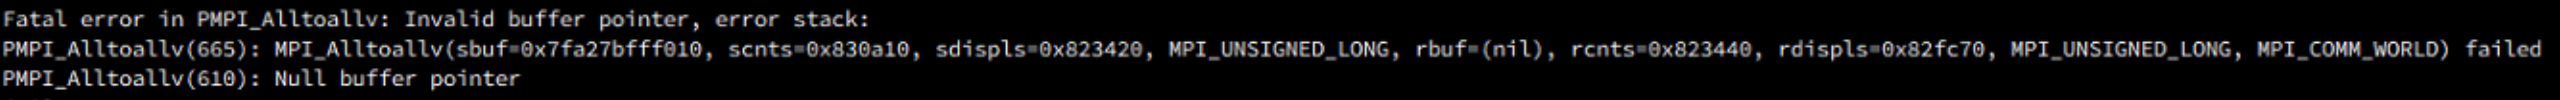
\includegraphics[scale=0.3]{assets/error.png}
    \caption{运行错误时的报错截图(请放大来看)\label{fig:error}} 
    \end{center} 
\end{figure} 

\begin{figure}[!hbt]
\begin{itemize}
\item[] \begin{lstlisting}[style=mycpp, label=lst:error, caption=报错代码展示]
ul_t* my_swap_array = (ul_t*) malloc(sizeof(ul_t) * my_recv_count);

MPI_Alltoallv(my_array, send_count_array, sdispls_array, MPI_UNSIGNED_LONG,
    my_swap_array, all_count_array, rdispls, MPI_UNSIGNED_LONG, MPI_COMM_WORLD);
\end{lstlisting}
\end{itemize}
\end{figure}

% \begin{appendices}
% \section{参考文献} \label{sec:reference}
% \section{伪代码补充} \label{sec:file}

% \end{appendices}
\end{document}
